\section{第二章~~~~~~~曲面和微分几何}

微分几何是对曲面(流形)形状的详细研究,包括局部和全局性质。$\mathbb{R}^3$(三维)中的平面是一个非常简单的曲面,不需要特殊的工具来描述它。另一方面,一个“任意”形状的表面,如汽车的引擎盖,有许多明显的几何特征。(高度弯曲区域、几乎平的区域等)。定量和定性地描述这些特征需要微分几何的工具。此外,几何细节在许多物理和生物过程中都很重要,例如表面张力$[20,21]$和生物膜$[9,55,90,114]$。

微分几何的框架首先通过定义一个局部映射(如,曲面参数)。然后,在曲面上建立了一个类似于标准“欧几里德微积分”的微积分框架。也可以采用其他方法,例如使用由级别集(level sets)和距离函数定义的隐式曲面。尽管是任意的,但是参数化在各种设置中都非常有用,所以我们将主要使用这些。我们强调曲面的几何形状不依赖于特定的参数化;在$2.3$节中引入正则曲面的概念来处理这个问题(参见命题$1$)。
在这一章以及本书的其余部分,我们主要关注三维空间中的二维曲面。我们首先回顾一些基础知识,以便使本文尽可能完整。

\subsection{预备}
下面几节将快速回顾本书的基本概念。然而,为了阅读本书,理解集合、映射等的所有细节并不重要。但是,如果这里讨论的观点与您完全不同,那么我们鼓励您参考一本好的教科书,如[61,62,64]
\subsubsection{欧几里得空间}
$\mathbb{R}^n$表示$n$维欧氏空间。在整个文本中,我们主要取$n=3$,但有时我们可能会专门化成$n=2$。我们假设读者熟悉笛卡尔坐标系、向量符号和向量算法、向量运算点积、叉乘、两个向量之间的夹角等。$\mathbb{R}^3$中的一般向量$\mathbf{x}$通常有由$\mathbf{x}= (x_1, x_2, x_3)$表示。

接下来,假设我们有一个给定的坐标系。任何点$P$在$\mathbb{R}^n$中都有一个唯一的位置向量,即$\mathbf{x}_P\in \mathbb{R}^n$,它从原点到$P$。点$P$的坐标就是向量$\mathbf{x}_P$的分量。因此,有时用向量$\mathbf{x}_P$来表示点$P$是很方便的,这意味着我们将通过位置矢量来表示该点。这种情况下,我们将去掉下标,只引用点$\mathbf{x}$。当没有歧义的时,我们将充分使用这种符号。否则,我们将强调点和位置向量之间的区别。
\subsubsection{开闭集合,边界,领域}
一般来说,集合是不同对象的集合。例如,$\lbrace  X,Y \rbrace$是由不同的对象$X$和$Y$组成的集合;我们在定义一个集合时使用大括号$\lbrace  , \rbrace$。我们经常引入另一个符号,如$Q=\lbrace X , Y \rbrace$,为了方便引用集合。设$S$和$U$为集合,它们之间存在关系有交集,补集,并集等。

有时候一个集合是通过一个条件定义的。例如,$ \lbrace x\in G$:$x$要满足条件$\rbrace$,例如集合$\lbrace 1,2,3\rbrace$也可以由$\left\{ a \in \mathbb{Z}:a>0~and~a<4  \right\}$定义,其中$\mathbb{Z}$是整数集。空集表示为$\emptyset $,是唯一一个没有元素的集合:$\lbrace  ~ \rbrace$。

给定$\mathbb{R}^n$中一个点$\mathbf{x}$,和一个正数$r$,设$B_r(\mathbf{x})$是$\mathbb{R}^n$中所有到点$\mathbf{x}$的距离严格小于$r$的集合,表达如下
\begin{gather}
B_r(\mathbf{x})=\left\{ \mathbf{y} \in \mathbb{R}^n:\left| \mathbf{x} - \mathbf{y} \right| <r \right\}
\end{gather}
换句话说,$B_r(\mathbf{x})$是一个以$\mathbf{x}$为中心半径为$r$的实心球($n$维)的内部。接下来,我们定义$B_r(\mathbf{x})$的边界为
\begin{gather}
\partial B_r(\mathbf{x})=\left\{ \mathbf{y} \in \mathbb{R}^n:\left| \mathbf{x} - \mathbf{y} \right|=r  \right\}
\end{gather}
即$\partial B_r(\mathbf{x})$是以$\mathbf{x}$为中心半径为$r$的球面。
从上面我们可以看到$B_r(\mathbf{x}) \cap \partial B_r(\mathbf{x})$是空集,$B_r(\mathbf{x})$不包含$\partial B_r(\mathbf{x})$的任何部分。换句话说,$B_r(\mathbf{x})$不包含其边界的任何部分。更正式的写法是$B_r(\mathbf{x}) \cap \partial B_r(\mathbf{x})=\emptyset$。

我们使用术语$open$表示一个集合不包含其边界的任何部分。更准确地说,一个子集$U$在$\mathbb{R}^n$是开的,如果$U$中每个点都有$B_r(\mathbf{x})$,其中$r>0$,且包含在$U$中。换句话说,给开集$U$中一点$\mathbf{x}$,我们可以找到一个包含$\mathbf{x}$的球完全包含在$U$中。事实上,我们经常把$B_r(\mathbf{x})$看成一个开球。另一个开放集的例子是$(0,1)\subset R$ 。 即$0$和$1$之间的组数,但不包括$0$和$1$。

一个$S\in \mathbb{R}^n$的集合的边界是$\mathbb{R}^n$中的点,使得包含此点的开集即包含有$S$中的点又包含有不是$S$中的点。换句话说,$S$中边界点$\mathbf{x}$,对于任意$r$,都满足$B_r(\mathbf{x}) \cap S\neq \emptyset$和$B_r(\mathbf{x}) \cap (\mathbb{R}^n \ S)\neq \emptyset$。我们用$\partial S$表示$S$的边界,参见图$2.1$的图形说明。
\begin{figure}[H]
\centering
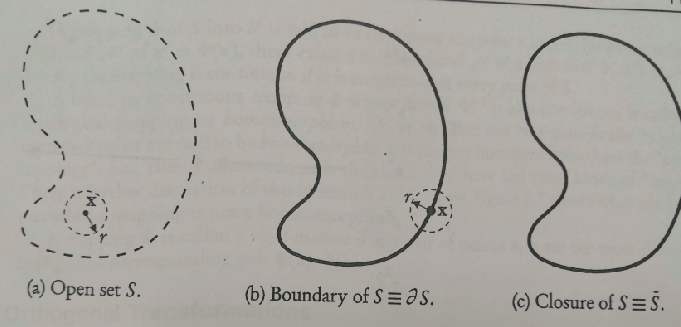
\includegraphics[scale=0.5]{./figures/21.png}
\caption{}
\end{figure}

我们用闭的说明集合包含所有边界,沿着这些线,用$\bar{S}$表示$S$的闭包,等于$\bar{S}=S \cup \partial S$。因此我们有一个以$\mathbf{x}$为圆心,半径为$r$闭合球$\overline{B_r(\mathbf{x})}$表示为
\begin{gather}
\overline{B_r(\mathbf{x})}=\left\{ \mathbf{y} \in \mathbb{R}^n:|\mathbf{x}- \mathbf{y}| \leq r \right\}
\end{gather}
另一个闭集例子$[0,1]\subset \mathbb{R}$,这个闭集即包含$0$到$1$之间的数,又包含$0$和$1$。

\textbf{备注2.}在这本书中,我们经常围绕一个点来定义一个领域,如,点$\mathbf{x}$的邻域,是任何包含$\mathbf{x}$的开集$U \subset \mathbb{R}^n$。

\subsubsection{紧集}
如果一个集合包含在$\mathbb{R}^n$中一个足够大但半径有限的开球中,那么它就是有界的。此外,如果$\mathbb{R}^n$中的集合是闭的和有界的,那么它就是紧集。紧性的概念实际上比这更普遍[63,64]。但是对于我们的目的,前面的定义是充分的。

如果$\bar{S} \subset W$和$\bar{S}$是紧的,我们说一个(非空)开集$S$紧包含在另一个开集$W$中,记为$S \subset \subset W$。也就是说,$S$的边界不能与$W$的边界接触,即,在$\partial S$和$\partial W$之间有“一点空间”。有了这个,我们现在可以证明紧支撑函数的概念。假设$f$是定义在$S$上的函数,$f$的支撑被定义为$S$中$f$的函数值非零的点的集合。
$$supp (f)= \left\{ \mathbf{x} \in S :f(\mathbf{x}) \neq 0 \right\}$$
此外,如果$\overline{supp (f)} \subset \subset S$,我们就说$f$是$S$中紧支撑。
\begin{figure}[H]
\centering
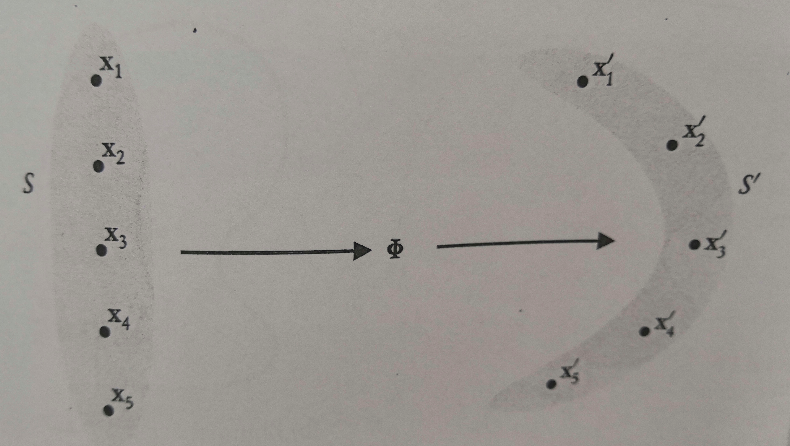
\includegraphics[scale=0.5]{./figures/22.png}
\caption{$\mathbb{R}^n$中的集合$S$通过映射$\Phi$映射到$S^{'}$上。对于$i=1,...,5$这些点对应于$\mathbf{x}_i^{'}=\Phi(\mathbf{x})$。我们可以把$\Phi$的作用解释为集合$S$变形为$S^{'}$,也就是说,$S$通过变换$\Phi$变成$S^{'}$的形状。}
\end{figure}

\textbf{备注3.}紧支持是忽略边界的有用影响。对于本书中的一些证明,我们需要这个概念来保持“一个泛函的作用”远离一个集合的边界,或者在一个感兴趣的区域内局部化一个函数。一个原因是为了避免在定义的边界上函数进行微分会产生潜在的差异。或者,更常见的是,我们希望忽略一个依赖于函数在边界点的值的量。例如,如果$f$在$S$上有紧支撑,则$\int _{\partial S}f=0$。

\subsubsection{映射:基本定义}
$S$和$S^{'}$是两组集合。如果有一个“规则”(函数)$\Phi$,使$S$中的每一点都有$S^{'}$中的点$\mathbf{x}^{'}$与之对应,则我们说这是一个集合$S$到$S^{'}$的映射或变换。我们使用符号$\Phi$:$S\rightarrow S^{'}$表达前面语句的简称。
有了这个,我们可以写成$\mathbf{x}^{'}=\Phi (\mathbf{x})$我们称$\mathbf{x}^{'}$为$\mathbf{x}$的像点,$\mathbf{x}$称为$\mathbf{x}^{'}$的逆像点。

\textbf{备注4.}一般来说,如果$S\subset \mathbb{R}^m$和$S^{'}\subset \mathbb{R}^n$,则
\begin{gather}
\Phi =(\Phi _1,\Phi _2,...,\Phi_n)^T
\end{gather}
其中每个$\Phi _i$是一个$m$个参量的函数:$\Phi _i = \Phi _i(x_1,x_2,...,x_m)$。

$S$中所有点的像点集合称为$S$的像,记为$\Phi (S)$。如果$S^{'}$中每一点都是$S$中的像点,则映射$\Phi$将$S$映到$S^{'}$上,即$S^{'}=\Phi (S)$
。在这种情况下,我们称$\Phi (S)$为满射。参见图$2.2$是$\mathbb{R}^2$中的点集映射的一个例子(参见图$2.3$是$\mathbb{R}^3$一组映射的例子)。

如$S$中任意一对不同点的像点也是$S^{'}$中的不同点,那么我们称$\Phi (S)$是单射(也叫一对一映射)。$\Phi$即是满射又是单射(称为双射),则存在$\Phi$的逆映射,记$\Phi ^{-1}$,将$S^{'}$中的点映射到$S$上。即如果$\mathbf{x},\mathbf{x}^{'}$满足$\mathbf{x}^{'}= \Phi (\mathbf{x})$,则$\mathbf{x}=\Phi ^{-1} (\mathbf{x}^{'})$,$\Phi ^{-1} :S^{'}\rightarrow S$

$S$到$S^{'}$的映射$\Phi$在$S$中的$\mathbf{x}$点处是连续的,如果对于任意包含$\mathbf{x}^{'}= \Phi (\mathbf{x})$的一个领域$N^{'}$,存在$\mathbf{x}$的一个领域$N$,使得$\Phi (N)\subset N^{'}$。如果它在$S$的每一点都是连续的,我们称该映射是连续的。

双射$\Phi$是连续映射,并且其逆$\Phi^{-1}$也是连续的,则称为拓扑映射或同胚。点集可以拓扑地互映射到其他点集称他们为同胚的。同胚集合具有相同的“拓扑”,即,它们的连通性是一样的;它们有相同类型的“洞”。在$2.3.1$节中对此有进一步的讨论,图$2.7$显示了当映射不是同胚时可以发生什么。

如果任意两点$\mathbf{a}$和$\mathbf{b}$的距离等于$\Phi(\mathbf{a})$和$\Phi(\mathbf{b})$的距离,映射$\Phi$就称为刚性运动(rigid motion)。

\subsubsection{正交变换}
设$b = (b_1, b_2, b_2)\in~\mathbb{R}^3$,$A\in~\mathbb{R}^{3\times 3}$,即一个$3\times 3$矩阵$A=[a_{ij}]_{i,j=1}^3$,$a_{i,j}$是矩阵$A$的元素。定义以下(仿射affine)线性映射$\Phi$(转换):
\begin{gather}
\tilde{\mathbf{x}}=\Phi (\mathbf{x})=A\mathbf{x}+b~~~~~~~~\Leftrightarrow~~~~~~~~\tilde{x_i}=\Phi (\mathbf{x})_i=\left( \sum _{k=1}^{3}a_{ik}x_{k} \right)+b_i,
\end{gather}
这里$(\Phi(\mathbf{x}))_i\equiv \Phi _i(x_1,x_2,x_3)$。如果$A$满足下面性质
\begin{gather}
A^{-1}=A^{T},~~~~~~~~~det(A)=1,
\end{gather}
其中$det(A)$为$A$的行列式,则$\Phi$表示刚体运动。基本上,$\Phi$由一个旋转(rotation)($A$),后跟一个转变(translation)($b$)。一个刚性运动可以被用来从一个笛卡儿坐标系统转换到另一个坐标系。

如果$b=0$并且$(2.6)$仍然成立,则$\Phi(\mathbf{x})=A\mathbf{x}$是一个线性映射称为正交变化(direct orthbogonal transformation)。这不过是以原点为中心的坐标系的旋转。如果$(2.6)$被替换为
\begin{gather}
A^{-1}=A^{T},~~~~~~~~~det(A)=-1,
\end{gather}
则$\Phi(\mathbf{x})=A\mathbf{x}$称为反正交变换,$(2.6)$和$(2.7)$都是正交矩阵的。\\

\textbf{备注4(转换的解释).}我们可以用两种不同的方法来解释$(2.5)$。考虑$\\mathbb{R}^3$坐标为$\mathbf{x}$的点$P$。\\

$\bullet$Alias.将$(2.5)$作为坐标的变换,$\mathbf{x}$和$\tilde{\mathbf{x}}$是相对于不同坐标系同一个点的坐标。换句话说,该点由不同的“名称”。\\

$\bullet$Alibi.将$(2.5)$看成集合的映射,$\mathbf{x}$和$\tilde{\mathbf{x}}$是同一坐标系下不同点的坐标。换句话说,点$\tilde{\mathbf{x}}$是点$\mathbf{x}$映射之前的点。

质点(material)的概念与alibi的观点直接相关,我们可以想象一个物质的“粒子”(即质点),最初在$\mathbf{x}$,然后因为某种物理过程而转移到$\tilde{\mathbf{x}}$点。转换$(2.5)$简单地表示物理过程的运动结果。在变形连续介质力学中是标准概念,尤其是非线性弹性力学中。图$2.3$是$\mathbb{R}^3$中点集的一个刚体运动。

\begin{figure}[H]
\centering
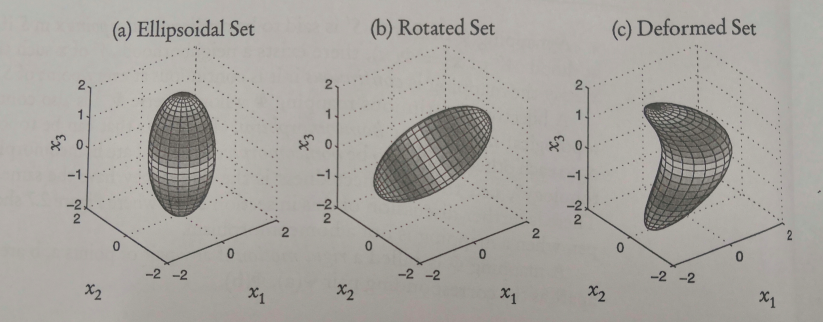
\includegraphics[scale=0.5]{./figures/23.png}
\caption{$(a)$是$\mathbb{R}^3$中点集$S$。$(b)$是$S^{'}=\Phi (S)$的旋转集合,其中$\Phi$是$(2.5)$和$(2.6)$中定义的。$(c)$是$S^{'}=\Phi (S)$的变形集合,其中$\Phi$是$(2.9)$中定义的。}
\end{figure}

\subsubsection{一般的变换}
一般来说,变换可能不是线性的。因此,$\Phi$:$\mathbb{R}^3 \Rightarrow \mathbb{R}^3$可能写成
\begin{gather}
\Phi=(\Phi _1,\Phi _2,\Phi _3)^T,
\end{gather}
这里,$(\Phi_i= \Phi _i(x_1,x_2,x_3) (i = 1,2,3)$为标量值(非线性)函数。备注$5$也适用于这些转换。因此,alias的观点生成一个曲线坐标系。alibi观点意味着集合$S$变形为$S^{'}=\Phi (S)$。如图$2.3$所示,非线性映射被应用于椭球形点集的例子,其中$\Phi$定义为
\begin{gather}
\Phi=(x_1-1.2+1.6\cos (x_3 \pi /4),x_2,x_3)^T.
\end{gather}

当处理从$\mathbb{R}^n$映射到$\mathbb{R}^n$的变换时,我们将使用符号$\Phi$来表示变换(通常$n =2$或$3$),但是我们也将考虑从$\mathbb{R}^q$到$\mathbb{R}^n$的变换,其中$q <n$。当$q = 2$和$n = 3$时,我们用转换$X$:$\mathbb{R}^2 \Rightarrow \mathbb{R}^3$,我们使用不同的符号去表示;在定义曲面时使用这(参见$2.2.1$和$2.3$节)。注意,我们可以把$X$看作$\Phi$是对$x_1,x_2$平面的限制。当$q = 1$时,我们使用符号$\alpha$:$\mathbb{R}^1 \Rightarrow \mathbb{R}^n$,$n=2,3$,这对应于参数化曲线。类似地,我们可以把$\alpha$看成是$\Phi$对$x_1$轴的限制。